%%%%%%%%%%%%%%%%%%%%%%%%%%%%%%%%%%%%%%
% yale_thesis.tex
% Alexander Cerjan
% 2014/04/07
%
% A bare, sample template for a Yale PhD thesis using yalephd.cls
%%%%%%%%%%%%%%%%%%%%%%%%%%%%%%%%%%%%%%

\documentclass[letterpaper,11pt]{yalephd}
% remove draft option for final printing.
% font size must be between 10pt-12pt.

\usepackage{geometry} % you need this for yalephd.cls to work.
\usepackage{graphicx} % you probably want the rest of these.
\usepackage{dcolumn}
\usepackage{bm}
\usepackage{amsmath}
\usepackage{amsfonts}
\usepackage{amssymb}
\usepackage{appendix}
\usepackage{comment}
\usepackage{cite}
\usepackage{notoccite}

\bibliographystyle{abbrvunsrt}

\begin{document}

% Need to define title before the abstract.
\title{Title goes here}
\author{Your name}
\advisor{Your advisor's name}
\date{Month, year you'll receive your degree, like ``May, 2015''} % usually not \today.

% All the stuff at the front of your thesis.
\frontmatter

\begin{abstract}
Abstract goes here. Limit 750 words.
\end{abstract}


\maketitle
\makecopyright{2015} % change as needed.
\tableofcontents
\listoffigures % remove this if you have no figures.
\listoftables % remove this if you have no tables.

\chapter{Acknowledgements} % this needs to be before \mainmatter.
A lot of people are awesome. Probably your family, friends, 
advisor, and that one super special high school teacher who
believed in you.

% Starts proper arabic numbering of pages and chapters.
\mainmatter

\chapter{Introduction}
Your first chapter is probably an introduction. But who knows. Check out Eq.\ (\ref{that_right_triangle_rule})!
Note that after Eq.\ and Fig.\ you want to use `.\textbackslash'  to use a single sized space. Otherwise,
latex will interpret it as the end of a sentence and put additional white space in between `Eq.' and 
`(\ref{that_right_triangle_rule})'.

\begin{equation}
a^2 + b^2 = c^2 \label{that_right_triangle_rule}
\end{equation}

The Physics Department recommends that the first chapter of the thesis be 
a succinct summary of the entire thesis, including in particular:

\begin{enumerate}
  \item a brief review of the field prior to the thesis research to provide context
  \item a presentation of the goals and motivations of the thesis research 
  \item a clear description of what the student has achieved in the thesis research
 (primarily written in the first person singular, but with due credit to
 others as appropriate). This description should refer back to (1) and clearly indicate the relation
 to prior work.
\end{enumerate}
It may also make sense to add suggestions for how to best build upon the thesis research in future work. Otherwise these suggestions should appear in the conclusion of the thesis.


\chapter{A new chapter}
Your second chapter probably has novel material in it. hopefully.

% Add additional \chapter{}s as necessary.

% use \cite{} to cite a reference in your bibliography file.
% use \ref{} to reference a \label{} from an equation, figure, or table.

% for sets of equations use align or gather:
%\begin{align}
%\end{align}

% for long equations, use multline.

% for figures:
%\begin{figure}[ht]
%\centering
%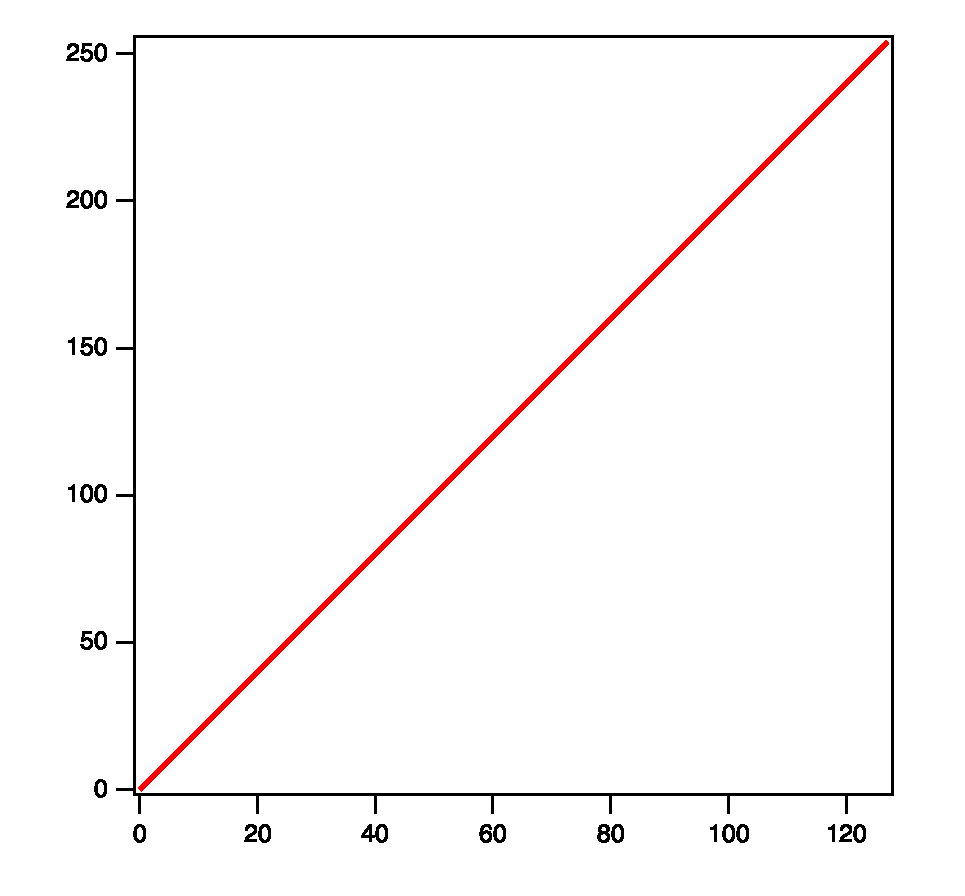
\includegraphics[width=.45\textwidth]{name_of_figure.eps}
%\caption{A caption! \label{a_figure}}
%\end{figure}

% for tables:
%\begin{table}
%\begin{tabular}{c|c|c}
% 1 & 2 & 3 \\
%\hline
%\end{tabular}
%\caption{Another caption! \label{a_table}}
%\end{table}

% Only call appendix once, here.
\appendix

\chapter{Stuff}
If you need an appendix, it will go here.

\begin{align}
a^n + b^n &\ne c^n \\
n &> 2
\end{align}

\chapter{More stuff}
A second appendix. Look at you, you over achiever.

% Any chapters such as End Notes go after this.
\backmatter

\bibliography{name_of_your_bibtex_file}
% for your own sake, use a bibtex file, so all of the numbering of references will be done
% automatically.

\end{document}
